Social media is a term referring to online communication channels meant for social interaction, content-sharing and collaboration. Over time, this term became widely used, its exact definition somewhat blurred and if really wanted, most of the today's websites could be labeled as social media. In context of this thesis,  I refer to social media in its “original” meaning. To be considered a social media platform, most of following features usually need to be fulfilled:

\begin{itemize}
  \item \textbf{User accounts} - platform allows users to create and run their own accounts that they can log into. These are online representations of their owners and serve as a too to reach and interact with other users.
  \item \textbf{Profile pages} - pages which represent an individual, might it be a real person, group of people or company. It should contain several personal information about the user like bio, profile picture or some other personal data.
  \item \textbf{Friends, followers, groups} - list of accounts whose owners have some form of a relationship  or common interest with the user.
  \item \textbf{News feeds} - Area where all new content from other connected entities appears.
\end{itemize}

Even if a platform fulfills these requirements, it doesn't necessarily have to be classified as social networking platform as pointed out in Haewoon Kwak's paper\cite{kwak2010twitter}.

\section{Potential of social media data mining}
Social media are changing the way that information is passed across societies and around the world.\cite{mayfield2008social}
Among many other potentials of social media, there is a huge amount of data generated on daily basis. These data carry lots of real world data and if used correctly, can offer deep insight into almost any area. The process of analyzing these data and searching for repetitive reoccurring patterns with goal of predicting future trends is also called social media mining. Successful mining can not only save money and time spent on getting the data in more traditional way like surveys but can also provide crucial factor in planning or decision making of businesses. Although internet is one big hole and contains lot of false facts and desinformation, there is indication that social networks tend to favour
valid information over rumours.\cite{castillo2011information} 

\section{Data}
\subsection{Getting data} \label{ssec:GettingData}
As you will have a chance to see, big social networking platforms started realizing that data they own are a “golden egg” and getting raw full data from them got much more difficult than it was in the early years of social media age.

\paragraph{Twitter:}
When talking about sentiment analysis of social media, analysis of Twitter data has in last couple of years became almost a default choice. This change can be nicely seen in the Mantyla, Graziotin and Kuutila's \cite{mantyla2018evolution} wordcloud of SE papers before and after 2013.\ref{fig:papersWordcloudHistory}.

\begin{figure}[H]%
    \centering
	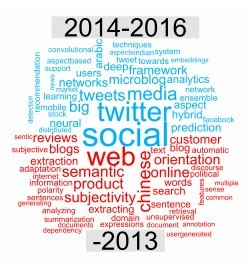
\includegraphics[width=8cm]{papersWordcloudHistory.jpg}
    \caption{Wordcloud comparison of pre and post 2013 SE papers \ref{fig:papersWordcloudHistory}}%
    \label{fig:papersWordcloudHistory}%
\end{figure}

To get the data from Twitter,  I first tried to use the Twitter API but I very early got to know that Twitter is well aware of the worth of their data. They do not provide tweets older than 2 weeks what basically made their API inapplicable for my purposes. The only way how to get historical Twitter data is actually:

\begin{itemize}
  \item collect them over time
  \item buy them from Twitter
  \item buy them from other companies who collect Twitter dumps over time
\end{itemize}

Therefore to obtain my data, I had to use the Twitter Search Api. To do this I used the GetOldTweets\footnote{https://github.com/Jefferson-Henrique/GetOldTweets-python} repository from Jefferson-Henrique which provides an extra layer on top of Search Api and simplifies working with it. Using this technique, I managed to get the significant amount of data needed for all my tasks in this thesis.\\
This repository offers following collection of search parameters which can be used to filter specific tweets according:
\begin{itemize}
  \item setUsername - Twitter account without "@"
  \item setSince - lower date bound with format "yyyy-mm-dd"
  \item setUntil - upper date bound with format "yyyy-mm-dd"
  \item setQuerySearch - search text to be matched
  \item setTopTweets - boolean flag whether to return only top tweets
  \item setNear - location are reference 
  \item setWithin - radius from "near" location
  \item setMaxTweets - max amount of tweets to be retrieved
\end{itemize}


I got historical Twitter data by looping all projects and their release dates and requested data: 

\begin{itemize}
  \item on the release dates (Listing \ref{lst:onReleaseDatesScript})
  \item in the interval of 2 days before and after  release date (Listing \ref{lst:beforeAfterReleaseDatesScript})
  \item weekly
\end{itemize}


\begin{lstlisting}[caption={Creating command to get Tweets about a project version on release dates},label={lst:onReleaseDatesScript},language=Python]
miningConsoleCommand = "python Exporter.py 
				--querysearch '" + frameworkName + " AND " + version + "'    --since " + str(releaseDate) + " 
				--until " + str(afterRelease) + " 
				--output='" + frameworkName + "_" + str(releaseDate) + ".csv" + "'"
\end{lstlisting}


\begin{lstlisting}[caption={Creating command to get Tweets about a project version in particular time interval around release date},label={lst:beforeAfterReleaseDatesScript},language=Python]
miningConsoleCommand = "python Exporter.py 
				--querysearch '" + frameworkName + "' 
				--since " + str(fromDate) + " 
				--until " + str(toDate)  + " --lang " + "en" + " 
				--maxtweets " + str(TWEETS_PER_RELEASE) + " 
				--output='" + frameworkName + ".csv" + "'"
\end{lstlisting}


\paragraph{Facebook:}
I originally planned to use Facebook statuses as a big part of analyzed data. Sadly, this was not possible since Facebook Graph API does not allow post searching feature. There was this option till early 2014 with Facebook API 1.x versions but since Graph API has been introduced, there is no way how to make Facebook application send requests to 1.x versions of API. At first, application created before 2014 were still working on top of the early Api versions and it has been maintained but over time, all the applications were migrated to 2.x Api versions. There is currently no public way how to freely get the Facebook posts data. The other types provided by the Api are for example user, page, event, group or place.

\paragraph{Reddit:}
Despite that reddit does not offer big amount of user data in OSS projects subreddits, I thought getting and working with Reddit could increase the variety of users and the data which I will be working with. To get the data I used Python Reddit API Wrapper (PRAW) used to directly work with Reddit Api via HTTP requests.\\
Class Reddit provides a convenient way how to access Reddit API. Instance of this class can be seen as a gateway to interact with API through PRAW. To instantiate this class, user first has to register his application. This gives user unique \textit{useragent} key which identifies the application. This is so that if a program misbehaves for some reason, it can be more easily identified, rather than look like a browser. All mandatory arguments are shown in Listing \ref{lst:redditClassInstance}.
\newpage
\begin{lstlisting}[caption={Instantiating Reddit class object},label={lst:redditClassInstance},language=Python]
reddit = praw.Reddit(
							clientid='CLIENTID',
							clientsecret="CLIENTSECRET", 				
							password='PASSWORD',
							useragent='USERAGENT',
							username='USERNAME'
							)
\end{lstlisting}

After connection to Api is successful, senting requests with PRAW is straightforward. To get the submissions from a particular subreddit in a specific time interval, just a basic loop shown in Listing \ref{lst:redditSubmissionsLoop} is enough.

\begin{lstlisting}[caption={Getting posts from subreddit *},label={lst:redditSubmissionsLoop},language=Python]
for submission in reddit.subreddit(redditName).submissions(FROM, TO)):
\end{lstlisting}
\textit{*During the writing of this thesis, new Reddit API deprecated the submission class and all endpoints using this class.}\\
\\
Each post (submission) contains among other information also array-like member variable of all comments. Simply concatenating all those gives the whole textual representation of the discussion.


\paragraph{Stack overflow:}
To extract the questions about the OSS projects of my interest I once again used provided Api. Python module called StackApi offers a way how to communicate with various Stack Exchange Api endpoints - answers, badges, comments, posts, questions, tags and users. To initiate communication with StackAPi, one needs only to specify Stack webpage and choose an endpoint, tag, time interval and if needed also some other non-mandatory parameters. Afterwards, calling \textit{fetch} method starts returning questions. Snippet of how I got the data can be seen in Listing \ref{lst:stacktQuestionsLoop}

\begin{lstlisting}[caption={Getting Stackoverflow questions with StackApi},label={lst:stacktQuestionsLoop},language=Python]
	SITE = StackAPI('stackoverflow')
    	SITE.max_pages = 1;
    	while True:
    		questions = SITE.fetch(
    			'questions',
    			fromdate=date(2012, 5, 8),  # year,month,day
        		todate=date(2016, 4, 15),
        		tagged=project,
        		filter='withbody',
        		sort='creation',
        		page=page
         )
\end{lstlisting}

At first I intended to use the type “posts” which returns both, questions and answers, but later I have realized how huge amount of data SO contains.  The average count of questions using one of the examined projects names as a tag was around 150 000. Because of this, I had to find out how to filter just the questions with higher probability of talking about bugs. Since the questions on SO do not have any labels which I could use to my advantage like I did with Git issues, I decided to keep just the questions which mention a word “bug”. This still left me with considerable big dataset of 8143 questions to work with. Out of all properties of questions retrieved from questions endpoint, I decided to store and further work just with several of them – mainly its title and body since these two provide most of the semantic meaning.